\begin{figure}[htbp]
  \centering
  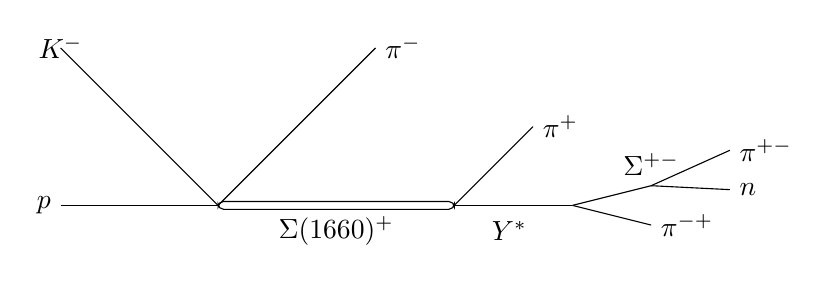
\begin{tikzpicture}
    \draw (-2.0, 2.0) node {$K^-$} -- (0, 0);
    \draw (-2.0, 0.0) node [left] {$p$} -- (0, 0);

    \draw (0, 0) -- (2.0, 2.0) node [right] {$\pi^-$};
    \draw (3.0, 0) -- (4.0, 1.0) node [right] {$\pi^+$};

    \draw [rounded corners=2pt] (0, 0.05) -- (3.0, 0.05) -- (3.0, -0.05) -- (0, -0.05) --cycle;
    \node (Sigma+) at (1.5, -0.33) {$\Sigma(1660)^+$};

    \draw (3.0, 0) -- (4.5, 0);
    \node (Y*) at (3.7, -0.33) {$Y^*$};

    \draw (4.5, 0) -- (5.5,  0.25) node [above] {$\Sigma^{+-}$};
    \draw (4.5, 0) -- (5.5, -0.25) node [right] {$\pi^{-+}$};

    \draw (5.5, 0.25) -- (6.5,  0.7) node [right] {$\pi^{+-}$};
    \draw (5.5, 0.25) -- (6.5,  0.2) node [right] {$n$};
  \end{tikzpicture}
  \caption{Decay chain of $K^- p \rightarrow \pi^- \Sigma^+(1660) \rightarrow \pi^- \pi^+ Y^* \rightarrow \pi^- \pi^+ (\pi \Sigma)^0$}
\end{figure}
